% LSCM Paper Presentation - 10 minutes
% ECE 467/567 Computer Graphics, Fall 2026
\documentclass[aspectratio=169]{beamer}

% Theme
\usetheme{Madrid}
\usecolortheme{default}

% Packages
\usepackage[T1]{fontenc}   % proper accented characters (Lévy, Jérôme)
\usepackage{lmodern}
\usepackage{amsmath,amssymb}
\usepackage{graphicx}

% Custom colors
\definecolor{darkblue}{RGB}{0,51,102}
\setbeamercolor{structure}{fg=darkblue}

% Remove navigation symbols and footline
\setbeamertemplate{navigation symbols}{}
\setbeamertemplate{footline}{}

% Title page info
\title{Least Squares Conformal Maps for Automatic Texture Atlas Generation}
\subtitle{SIGGRAPH 2002}
\author{Presented by: Tanner Muscarella\\[0.3em]
\small Original Authors: Bruno L\'evy, Sylvain Petitjean, Nicolas Ray, J\'er\^ome Maillot}
\institute{ECE 467/567 Computer Graphics and CAD\\Fall 2026}
\date{November 5th, 2026}

\begin{document}

% ==============================================================================
% SLIDE 1: Title
% ==============================================================================
\begin{frame}
  \titlepage
\end{frame}

% ==============================================================================
% SLIDE 2: The Problem
% ==============================================================================
\begin{frame}{The Problem: Texture Mapping for 3D Paint Systems}

\begin{columns}[T]
\column{0.5\textwidth}
\textbf{Goal:} Paint high-resolution details on 3D models

\vspace{0.5em}
\textbf{Challenge:}
\begin{itemize}
  \item Need to map 3D surface $\to$ 2D texture space
  \item Surface must be cut into ``charts'' (disk topology)
  \item Each chart needs a parameterization
\end{itemize}

\vspace{0.5em}
\textbf{Prior methods:}
\begin{itemize}
  \item Require \alert{convex boundaries}
  \item Generate \alert{many small charts}
  \item Result: Seams, artifacts, hard to paint
\end{itemize}

\column{0.5\textwidth}
\centering
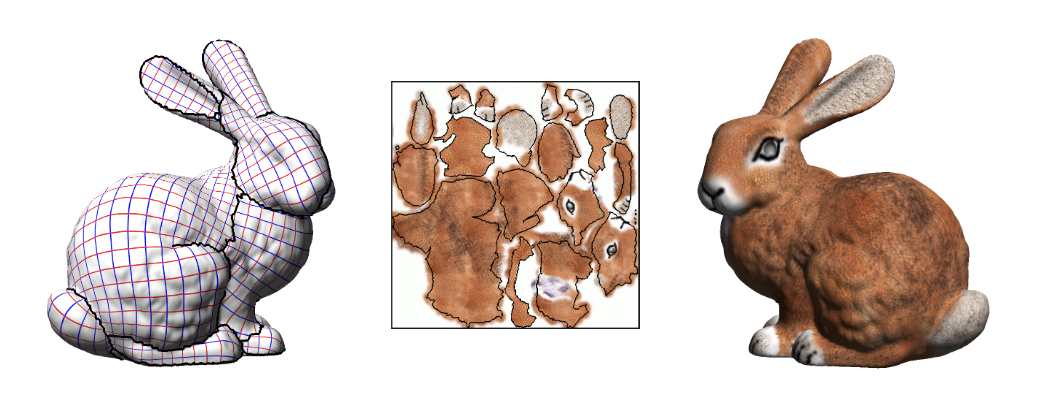
\includegraphics[width=0.95\textwidth]{fig_bunny_overview.png}

\vspace{0.3em}
\small\textit{3D model $\to$ UV charts $\to$ Textured result}

\end{columns}

\end{frame}

% ==============================================================================
% SLIDE 3: What is Conformal?
% ==============================================================================
\begin{frame}{Background: Conformal Mappings}

\begin{columns}[T]
\column{0.5\textwidth}
\textbf{Definition:} A map is \alert{conformal} if it preserves angles locally

\vspace{1em}
\textbf{Mathematically:}
\begin{itemize}
  \item Tangent vectors to iso-$u$ and iso-$v$ curves are:
  \begin{itemize}
    \item Orthogonal
    \item Same length
  \end{itemize}
  \item Cauchy-Riemann equations, with $U = u + iv$:
  \[
    \frac{\partial U}{\partial x} + i \frac{\partial U}{\partial y}
    = (u_x - v_y) + i\,(u_y + v_x) = 0
  \]
  i.e.\ $u_x = v_y$ and $u_y = -v_x$
\end{itemize}

\vspace{0.3em}
\textbf{Key insight:} Use complex numbers!

\column{0.5\textwidth}
\centering
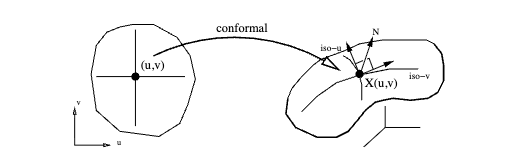
\includegraphics[width=\textwidth]{fig_conformal_concept.png}

\vspace{0.5em}
\small\textit{Figure 2: Conformal map preserves angles}

\vspace{1em}
\alert{Trade-off:} Cannot preserve both angles AND areas\\
unless the surface is developable (zero Gaussian curvature)\\
(Gauss's Theorema Egregium)

\end{columns}

\end{frame}

% ==============================================================================
% SLIDE 4: Comparison with Related Work (moved up to motivate LSCM)
% ==============================================================================
\begin{frame}{Prior Work: Why a New Method?}

\begin{block}{1. Harmonic Maps (Eck et al.\ 1995)}
\begin{itemize}
  \item \textcolor{red}{Requires convex boundary:} All boundary vertices fixed to convex polygon
  \item \textcolor{red}{Indirect coupling:} $u$ and $v$ solved in two separate linear systems
  \item \textcolor{green!50!black}{Fast:} Linear solve
\end{itemize}
\textbf{Limitation:} Cannot handle complex boundaries $\Rightarrow$ many small charts
\end{block}

\vspace{0.3em}

\begin{block}{2. MIPS (Hormann \& Greiner 2000)}
\begin{itemize}
  \item \textcolor{green!50!black}{Free boundary:} Allows complex borders
  \item \textcolor{red}{Non-linear optimization:} Expensive, local minima issues
  \item \textcolor{red}{No guarantees:} Uniqueness/triangle flips not proven
\end{itemize}
\end{block}

\vspace{0.3em}
\textbf{Goal of LSCM:} free boundary like MIPS, \alert{linear solve} like harmonic maps

\end{frame}

% ==============================================================================
% SLIDE 5: The LSCM Method
% ==============================================================================
\begin{frame}{The LSCM Method: Least Squares Approach}

\textbf{Key Idea:} Piecewise-linear maps can't satisfy Cauchy-Riemann exactly $\Rightarrow$ minimize the violation

\vspace{0em}
\begin{block}{Per-Triangle Criterion}
For each triangle $T$:
\[
  C(T) = \int_T \left| \frac{\partial U}{\partial x} + i \frac{\partial U}{\partial y} \right|^2 dA
  = \left| \frac{\partial U}{\partial x} + i \frac{\partial U}{\partial y} \right|^2 A_T
\]
\end{block}

\vspace{0em}
\begin{block}{Global Minimization}
Sum over all triangles:
\[
  C(\mathbf{U}) = \sum_{T \in \mathcal{T}} C(T) = \mathbf{U}^* \mathbf{C} \mathbf{U}
\]
where $\mathbf{C} = \mathbf{M}^* \mathbf{M}$ is a Hermitian Gram matrix
\end{block}

\textbf{Result:} Quadratic optimization $\Rightarrow$ \alert{Sparse linear system}\\
Pin $p \ge 2$ vertices $\Rightarrow$ unique solution; \alert{$p = 2$ is optimal} (developable $\Rightarrow$ zero distortion)

\end{frame}

% ==============================================================================
% SLIDE 6: Discretization (NEW)
% ==============================================================================
\begin{frame}{Discretization: Where the Complex Numbers Pay Off}

\begin{columns}[T]
\column{0.58\textwidth}
\setlength{\abovedisplayskip}{4pt}\setlength{\belowdisplayskip}{4pt}
\textbf{Per triangle} (local 2D frame, $U$ linear on $T$):
\vspace{0em}
\[
  \frac{\partial U}{\partial x} + i\frac{\partial U}{\partial y}
  = \frac{i}{d_T}\,\bigl(W_1U_1 + W_2U_2 + W_3U_3\bigr)
\]
\begin{itemize}
  \item $W_j$ = edge opposite vertex $j$ as a complex number: $W_1 = (x_3 - x_2) + i\,(y_3 - y_2)$; \ $d_T = 2A_T$
\end{itemize}

\textbf{Energy per triangle:}
\vspace{0em}
\[
  C(T) = \Big|\sum_j \frac{W_j}{\sqrt{d_T}}\,U_j\Big|^2
\]

\textbf{Stack one row per triangle:}
\vspace{0em}
\[
  m_{ij} = \frac{W_{j,T_i}}{\sqrt{d_{T_i}}}, \qquad
  C(\mathbf{U}) = \|\mathbf{M}\mathbf{U}\|^2 = \mathbf{U}^*\mathbf{M}^*\mathbf{M}\,\mathbf{U}
\]

\column{0.39\textwidth}
\begin{alertblock}{Why this matters}
\begin{itemize}
  \item \textbf{One} equation per triangle involves $u$ and $v$ \textbf{together}
  \item Harmonic maps: two separate systems, coupled only through the fixed boundary
  \item Direct coupling $\Rightarrow$ boundary can be \alert{left free}
\end{itemize}
\end{alertblock}

\setlength{\abovedisplayskip}{4pt}\setlength{\belowdisplayskip}{4pt}
\vspace{0.3em}
\textbf{Pin and solve with CG} (free $f$, pinned $p$):
\[
  \min_{\mathbf{U}_f} \bigl\| \mathbf{M}_f \mathbf{U}_f + \mathbf{M}_p \mathbf{U}_p \bigr\|^2
\]
\[
  \Rightarrow\; \mathbf{M}_f^*\mathbf{M}_f\,\mathbf{U}_f = -\mathbf{M}_f^*\mathbf{M}_p\,\mathbf{U}_p
\]

\end{columns}

\end{frame}

% ==============================================================================
% SLIDE 7: Why LSCM is Better
% ==============================================================================
\begin{frame}{Why LSCM is Better: Proven Properties}

\begin{block}{Four Mathematical Guarantees}
\begin{enumerate}
  \item \textbf{Unique Minimum} (for $p \ge 2$ pinned vertices)
  \begin{itemize}
    \item Cannot get stuck in local minima, unlike non-linear methods (MIPS, etc.)
  \end{itemize}

  \item \textbf{Similarity Invariance}
  \begin{itemize}
    \item Rotating, scaling, or translating the UVs doesn't change the optimum
  \end{itemize}

  \item \textbf{No Triangle Flips} (pinned vertices on the boundary)
  \begin{itemize}
    \item Orientation preserved: $\det(J) > 0$ for all triangles
    \item Global overlaps still possible if the boundary self-intersects
  \end{itemize}

  \item \textbf{Resolution Independent}
  \begin{itemize}
    \item Refining the mesh leaves the original vertices' UVs unchanged
  \end{itemize}
\end{enumerate}
\end{block}

\vspace{0.3em}
\textbf{Practical benefit:} \alert{Free boundary} (no convex polygon needed) + fast CG solve on a sparse system

\end{frame}

% ==============================================================================
% SLIDE 8: The Full Pipeline
% ==============================================================================
\begin{frame}{Complete Texture Atlas Generation Pipeline}

\begin{columns}[T]
\column{0.33\textwidth}
\centering
\textbf{1. Segmentation}

\vspace{0.5em}
\begin{itemize}
  \item Detect features (sharpest 5\% of edges)
  \item Seeds at points \emph{farthest} from features
  \item Charts grow until they meet at features
\end{itemize}

\vspace{0.5em}
$\downarrow$

\textit{Seams hidden where shading changes sharply}

\column{0.33\textwidth}
\centering
\textbf{2. Parameterization}

\vspace{0.5em}
\begin{itemize}
  \item Apply LSCM to each chart
  \item Pin 2 vertices (graph diameter)
  \item Split charts with overlaps or high area distortion
\end{itemize}

\vspace{0.5em}
$\downarrow$

\textit{UV coordinates per vertex}

\column{0.33\textwidth}
\centering
\textbf{3. Packing}

\vspace{0.5em}
\begin{itemize}
  \item ``Tetris'' algorithm using chart outlines
  \item Efficiency \alert{0.55--0.60} vs 0.37--0.51 for bounding rectangles
\end{itemize}

\vspace{0.5em}
$\downarrow$

\textit{Final texture atlas}

\end{columns}

\vspace{1em}
\begin{block}{Key Advantage}
LSCM's free boundary $\Rightarrow$ larger charts with complex shapes $\Rightarrow$ fewer discontinuities
\end{block}

\end{frame}

% ===========================================================================
% SLIDE 10: More Results
% ==============================================================================
\begin{frame}{Results: Texture Atlases}

\begin{columns}[c]
\column{0.48\textwidth}
\centering
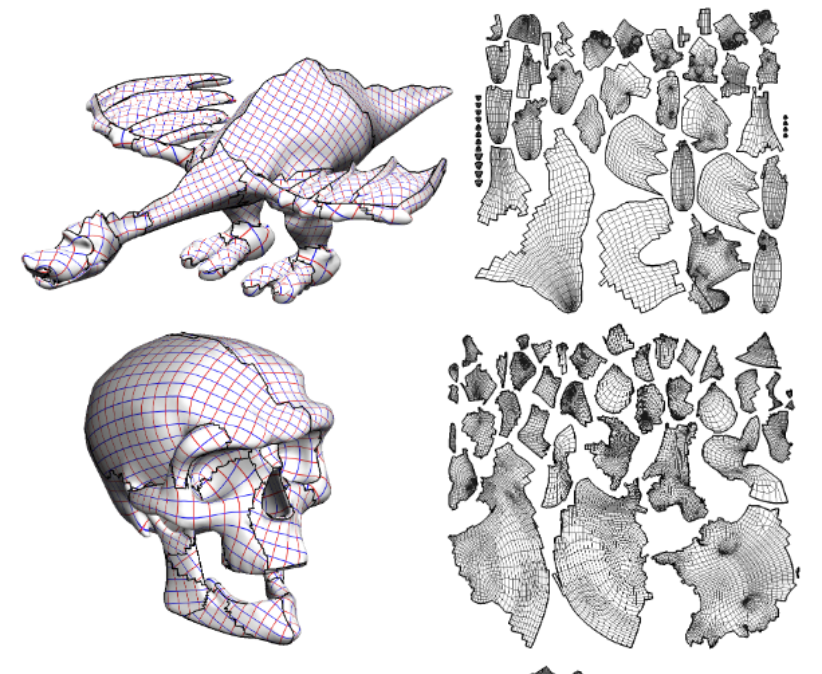
\includegraphics[width=\textwidth]{fig_results_atlas_pt1.png}

\column{0.48\textwidth}
\centering
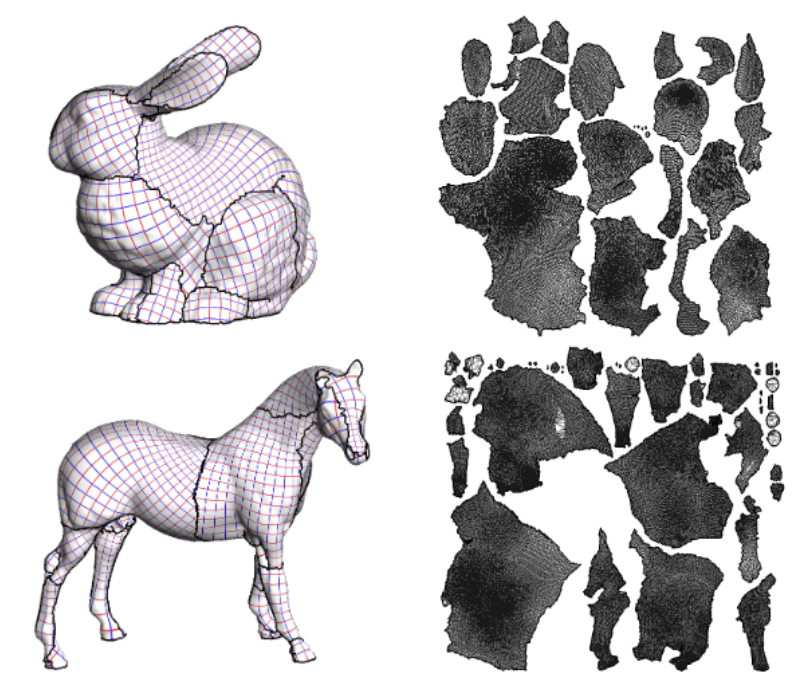
\includegraphics[width=\textwidth]{fig_results_atlas_pt2.png}
\end{columns}

\vspace{0.3em}

\begin{columns}[T]
\column{0.48\textwidth}
\small
Natural boundaries, low angle distortion
(angle between $\nabla u$ and $\nabla v$ peaks sharply at $90^\circ$)

\column{0.48\textwidth}
\small
Only 23--44 charts per model; boundaries follow features, easier painting
\end{columns}

\end{frame}

% ==============================================================================
% SLIDE 11: Impact & Limitations
% ==============================================================================
\begin{frame}{Impact and Limitations}

\begin{columns}[T]
\column{0.5\textwidth}
\textbf{Impact (20+ years later):}
\begin{itemize}
  \item \alert{Still widely used} in production
  \begin{itemize}
    \item e.g.\ Blender's ``Conformal'' UV unwrap
  \end{itemize}
  \item Building block for later methods:
  \begin{itemize}
    \item Common initialization for ARAP parameterization
    \item Multi-chart atlas generation
  \end{itemize}
  \item Integrated in tools:
  \begin{itemize}
    \item 3D paint systems
    \item Game engines
    \item Animation pipelines
  \end{itemize}
\end{itemize}

\column{0.5\textwidth}
\textbf{Limitations:}
\begin{itemize}
  \item \textbf{Area distortion:}
  \begin{itemize}
    \item Conformal $\Rightarrow$ high area variation
    \item Can fix with post-processing (stretch optimization)
  \end{itemize}

  \item \textbf{Overlaps possible:}
  \begin{itemize}
    \item If boundary self-intersects in UV
    \item Detected automatically
    \item Rare in practice
  \end{itemize}

  \item \textbf{Still needs cutting:}
  \begin{itemize}
    \item Charts must be disk topology
    \item Automatic segmentation helps
  \end{itemize}
\end{itemize}
\end{columns}

\end{frame}

% ==============================================================================
% SLIDE 12: Conclusion
% ==============================================================================
\begin{frame}{Takeaways}

\begin{block}{Three Key Contributions}
\begin{enumerate}
  \item \textbf{LSCM Parameterization:}
  \begin{itemize}
    \item Fast (sparse linear solve)
    \item Robust (unique solution, no flips)
    \item Flexible (free boundaries)
  \end{itemize}

  \item \textbf{Complex Number Formulation:}
  \begin{itemize}
    \item Direct coupling of $u$ and $v$ coordinates
    \item Elegant expression of Cauchy-Riemann
    \item Enables quadratic minimization
  \end{itemize}

  \item \textbf{Complete Pipeline:}
  \begin{itemize}
    \item Feature-based segmentation
    \item LSCM parameterization
    \item Efficient packing
  \end{itemize}
\end{enumerate}
\end{block}

\vspace{0.5em}
LSCM enables \alert{large charts with natural boundaries} $\Rightarrow$ better texture atlases for 3D painting

\end{frame}

\end{document}